\makeatletter

\section{Introduction}
We study the hypothetical scenario where the Perry Preschool Program (Perry) is applied to all U.S. children similar to those targeted by the original experiment. We investigate how this scenario would affect intra-black and black-white gaps in adult outcomes.  We follow \citet{heckman2010analyzing} to find the individuals in the National Longitudinal Survey of Youth 1979 (NLSY79) that are comparable to the participants of the Perry. Then, we utilize treatment effects from the Perry program and apply them to the comparable NLSY79 individuals. We refer to these individuals as \emph{disadvantaged}. This exercise permits us to learn how the gaps in relevant economic outcomes would look like had Perry been a national program. Particularly, we study: (i) the gap between disadvantaged and non-disadvantaged blacks (\emph{intra-black gap}) and (ii) the gap between blacks and whites (\emph{black-white gap}). 

The results show that the intra-black gap is considerably reduced for both men and women. For the case of men, however, the high school completion (no GED) completion gap goes up (253\%) because Perry had a negative treatment effect.\footnote{We argue that the negative effect of Perry on high school completion for men is a peculiarity of the location of the program. Ypsilanti, Michigan is a city near Detroit, which has a market for auto-parts that is a potential source of employment for high school dropouts. Perry could potentially lead to the following mechanism. Perry caused the individuals to have greater cognitive and non-cognitive abilities because the treated group seems to do better in a variety of outcomes other than high school completion. Importantly, Perry raised the marginal benefit of studying: future human capital builds on past human capital and treated individuals had more accumulated human capital when they decided attend high school or not. However, the opportunity cost of for abler individuals also goes up because the foregone earnings increase. If the latter increase is bigger than the former, abler individuals drop out of high school. The abler individuals, in this case, were the treated. Thus, the treatment effect of Perry was negative for the case of high school completion. This story is reinforced by the fact that, even when they attended less to high school, the individuals treated by Perry had higher employment probabilities and real incomes at ages 27 and 40.}. The gap is reduced in the rest of the outcomes: employment at 27 (59\%), labor income at 27(42\%), employment at 40(533\%), and labor income at 40 (55\%). For the case of women the gap is reduced in every outcome. The biggest reduction is in high school graduation at 27 (not including GED) (26,345\%), while the reductions in the rest of the outcomes are the following: employment at 27 (170\%), labor income at 27(34\%), employment at 40(48\%), and labor income at 40 (60\%). 

For the case of the black-white gap the results are lower in magnitude simply because the disadvantaged are a smaller fraction of the complete population than they are of the black population. The reductions for men are the following: employment at 27 (5\%), labor income at 27(3\%), employment at 40(24\%), and labor income at 40 (5\%). The high school completion gap has an increase (8\%), again, because the Perry program had a negative treatment effect for this outcome. For women, all the gaps decrease: high school graduation (not GED) (135\%), employment at 27 (44\%), labor income at 27(27\%), employment at 40(9\%), and labor income at 40 (18\%).

% matrix: AB file: tabp_perry.tex   3 Jul 2014 11:43:04
\begin{table}[htbp]
\caption{\label{tab:tabp_perry} Outcome Gaps after a Hypothetical Extension of the Perry Preschool Program to the Disadvantaged Black}\medskip
\footnotesize  \begin{center} \begin{tabular}{lcccccccccccccccccccccccc}  \hline \hline    
&\multicolumn{2}{c}{Scenario 1: No Action} &\multicolumn{6}{c}{Scenario 2: Disadvantaged Black Treated}  \\[0.05cm] \hline
 \textbf{(a) Female:} & \multicolumn{2}{c}{}   &  &\multicolumn{4}{c}{}   \\[0.02cm] 
\textbf{Individuals Treated} &\multicolumn{2}{c}{ 0 } &
 &\multicolumn{4}{c}{     376,015} &
 \\[0.2cm]  
\textbf{Cost of Intervention (2010 Mill.)} &\multicolumn{2}{c}{ 0 } &
 &\multicolumn{4}{c}{       7,222} &
 \\[0.2cm]  
\textbf{Gaps}&Intra-Black &Black-White & &Intra-Black &Change &Black-White &Change  \\[0.02cm] 
\hline
High School grad at 19 &       -0.01&        0.08&&       -0.57&        8902\% &       -0.01&        -114\% &
 \\[0.2cm]  
Employed at 27 &        0.15&        0.09&&       -0.13&        -191\% &        0.05&         -49\% &
 \\[0.2cm]  
Earnings at 27 (in 2010 dollars) &      11,352&       2,294&&       6,272&         -45\% &       1,452&         -37\% &
 \\[0.2cm]  
Employed at 40 &        0.02&        0.02&&        0.03&          48\% &        0.02&           9\% &
 \\[0.2cm]  
Earnings at 40 (in 2010 dollars) &       8,684&       4,563&&       1,991&         -77\% &       3,524&         -23\% &
 \\[0.2cm]  
\hline
 \textbf{(b) Male:} & \multicolumn{2}{c}{}   &  &\multicolumn{4}{c}{}   \\[0.02cm] 
\textbf{Individuals Treated} &\multicolumn{2}{c}{ 0 } &
 &\multicolumn{4}{c}{     375,077} &
 \\[0.2cm]  
\textbf{Cost of Intervention (2010 Mill.)} &\multicolumn{2}{c}{ 0 } &
 &\multicolumn{4}{c}{       7,204} &
 \\[0.2cm]  
\textbf{Gaps}&Intra-Black &Black-White & &Intra-Black &Change &Black-White &Change  \\[0.02cm] 
\hline
High School grad at 19 &        0.04&        0.08&&        0.02&         -48\% &        0.07&          -4\% &
 \\[0.2cm]  
Employed at 27 &        0.07&        0.15&&       -0.03&        -147\% &        0.13&         -11\% &
 \\[0.2cm]  
Earnings at 27 (in 2010 dollars) &       7,116&      16,780&&       1,554&         -78\% &      15,839&          -6\% &
 \\[0.2cm]  
Employed at 40 &        0.04&        0.15&&       -0.25&        -772\% &        0.10&         -35\% &
 \\[0.2cm]  
Earnings at 40 (in 2010 dollars) &      14,393&      27,626&&       5,477&         -62\% &      26,157&          -5\% &
 \\[0.2cm]  
\hline
 \textbf{(c) All:} & \multicolumn{2}{c}{}   &  &\multicolumn{4}{c}{}   \\[0.02cm] 
\textbf{Individuals Treated} &\multicolumn{2}{c}{ 0 } &
 &\multicolumn{4}{c}{     751,092} &
 \\[0.2cm]  
\textbf{Cost of Intervention (2010 Mill.)} &\multicolumn{2}{c}{ 0 } &
 &\multicolumn{4}{c}{      14,427} &
 \\[0.2cm]  
\textbf{Gaps}&Intra-Black &Black-White & &Intra-Black &Change &Black-White &Change  \\[0.02cm] 
\hline
High School grad at 19 &        0.02&        0.08&&       -0.27&       -1632\% &        0.03&         -60\% &
 \\[0.2cm]  
Employed at 27 &        0.11&        0.12&&       -0.08&        -177\% &        0.09&         -26\% &
 \\[0.2cm]  
Earnings at 27 (in 2010 dollars) &       9,234&       9,537&&       3,913&         -58\% &       8,646&          -9\% &
 \\[0.2cm]  
Employed at 40 &        0.03&        0.08&&       -0.11&        -479\% &        0.06&         -30\% &
 \\[0.2cm]  
Earnings at 40 (in 2010 dollars) &      11,539&      16,094&&       3,734&         -68\% &      14,841&          -8\% &
 \\[0.2cm]  
  \hline \hline    \end{tabular}
 \end{center} 
       {\scriptsize  
       {\raggedright 
{\bfseries Notes:} Panels (a), (b), and (c) present restults for female, male, and the overall population, respectively. The NLSY79 weights are used to make each sample representative of its corresponding in the population. Disadvantaged blacks meet the  Perry eligibility criteria. Non-disadvantaged blacks do  not. All blacks include disadvantaged and non- disadvantaged blacks and represent the U.S. population of blacks. All  whites represents the entire U.S. population of whites.  Scenario 1 is the baseline scenario, where Perry is not available. Scenario 2  makes the Perry Program available to all disadvantaged blacks. The intra- black gap measures the difference in adult outcomes between the non- disadvantaged black population and the disadvantaged black population.  The black-white gap compares the difference in adult outcomes between the  whole black population and the whole white population. The cost is expressed in 2010 millions of dollars. In the subsection that presents the gaps the first two columns display the actual gaps. The third column shows the gap after the treatment effects of Perry are applied to the disadvantaged black. The fourth column presents the the percentagae change between the first and the third columns. The fifth colum displays the black-white gap after the treatment effects of Perry are applied to the disadvantaged black.  The last column presents the the percentagae change between the fifth and the second columns.} } 
 \end{table}
 

We proceed as follows. First, we describe the impacts of the Perry Program and the study's participants. Second, we describe characteristics of the NLSY79 that allow us to understand the effect of the Perry Program if extended to the population. Finally, we present results.

\section{Treatment Effects of Perry}
The Perry Preschool Program was conducted in Ypsilanti, Michigan, a town near Detroit. It began in 1962. All of the study's participants were African-American and three years old at entry. The Perry children were randomized into control and treatment groups. The program gave treated participants access to a two-and-a-half hour, full-year preschool, five days a week for two years. Early on the program improved IQ, achievement and personality skills. These early impacts resulted in less crime, increased incomes and higher educational attainment in adulthood. Much work has traced the source and true magnitude of these treatment effects. We briefly describe the Perry sample both before and after the program. Then we discuss how to compute treatment effects and the source we use for the effects in our exercise. 

\subsection{The Perry Participants}
The Perry sample represents a group of very disadvantaged African-Americans. Compared to the general population in the 1960s, the Perry children suffered from disadvantage along several dimensions. They were born to mothers who, on average, achieved less than ten years of education. About half of the Perry families received welfare payments and had no father in the household. The children lived in large families, having on average five siblings. Such material disadvantage predicted poor development. The Perry children displayed signs of early cognitive delay, their Stanford-Binet IQ scores well below the population average. For most of these children, the future promised little chance of success. However, an experiment to assess the benefit of early intervention would give some of the young children an opportunity. The experiment provided another opportunity for researchers to test the impacts of high-quality preschool. 

\subsection{The Effect of the Perry Program}
Both groups were followed continuously from early childhood up until age 40. Despite their many disadvantages and early deficiencies, the intervention improved the lives of the treated individuals over their counterparts in the control group. About 65\% of treated group members graduated from High School compared to 45\% in the control group. At age 40, 76\% of the treated group were working compared to 62\% in the control group. Additionally, average earnings were nearly 33\% higher. The program sharply reduced negative behaviors as well. Treated group members committed fewer crimes and smoked less. 

Much literature focuses on the interpretation of treatment effects as causal effects. In particular, \citet{heckman2010analyzing} compute the causal effects of the Perry program on a variety of adult outcomes at ages 27 and 40. We utilize these effects to understand how a broader application of the program would affect the population. 

\subsection{Computing Treatment Effects}
The Perry Program is a randomized controlled trial (RCT). The assignment mechanism, $D$, is based on a random variable, $R$ and a vector of observable characteristics, $X$. The components of $X$ are IQ, entry cohort, socio-economic status, employment status of the mother, an indicator for elder sibling, and gender. Thus,
\[
D\sim M(R,X)
\]

\noindent The random variable, $R$, is independent of the vector of unobserved characteristics that determine treatment, $V$.  Then, 
\[
R\ci V
\]

\noindent Thus, the assignment mechanism is independent of potential outcomes $Y_{d}$, where the treatment is fixed at $d \in \{0,1\}$. Formally, under a RCT we have:

\[
 Y_d \ci D|X
 \]


\noindent Realized outcome can be written as follows:
\[
Y=DY_{1}+\left(1-D\right)Y_{0}
\]


\noindent Under a RCT we can identify the conditional Average Treatment Effect (ATE):
\begin{eqnarray*}
ATE(Y|X) = E[Y_1 = Y_0 | X]
\end{eqnarray*}

\noindent \citet{heckman2010analyzing} calculated treatment effects in this manner. After integrating over the distribution of observables $X$ they obtain ATEs separately for males and females. We apply these effects on comparable individuals in the NLSY79. But first we describe the feasibility of such an exercise with the NLSY79 data. 

\section{NLSY79}
In the previous section we discussed how to identify treatment effects conditional on observed characteristics. In this section we justify our exercise of imputing treatment effects to the NLSY79. The Perry and NLSY79 data share common support for most of the observed variables used in the Perry randomization protocol. Moreover, we note that the NLSY79 represents the young cohort of 1979, i.e., people aged 14 to 22, and, therefore, represents the national cohort to which the Perry individuals belonged. 

The NLSY79 Cohort is a longitudinal project that follows the lives of a sample of American youths born in the years 1957-1964. The individuals were interviewed for the first time in 1979, when they were between 14 and 22 years old. Two subsamples were dropped and 9,964 respondents remained. The data are now available for Round 1 (1979 survey year) and to Round 24 (2010 survey year). 

Three independent samples compose the NLSY79. These samples represent the entire population of youth aged 14 to 21 as of December 31, 1978, residing in the United States on January 1, 1979.  The three samples are: 1) A cross-sectional sample (6,111) designed to represent the non-institutionalized civilian segment of young people living in the United States in 1979 and born January 1, 1957, through December 31, 1964. 2) A supplemental sample (5,295) designed to oversample civilian Hispanic or Latino, black, and economically disadvantaged, nonblack/non-Hispanic youths born in the same time period. 3) A military sample (1,280) designed to represent the population born January 1, 1957, through December 31, 1961, serving in the military as of September 30, 1978. We asses the black-white and intra-black gaps with samples 1) and 2), respectively. 

The design of the first sample is as follows. Following the initial screening process, 6,812 individuals from the cross-sectional sample were designated to be interviewed in the base year; of those, 90 percent or 6,111 respondents were actually interviewed in 1979. Specifically, through the several stages of sample selection (counties, enumeration districts-block groups, sample listing units), probabilities of selection are based upon either total population or total housing units.  Except for the economically disadvantaged supplemental sample, sampling of nonblack/non-Hispanic respondents was restricted to the 102 PSU National Sample.

The design of the second sample is as follows. After screening, 5,969 individuals from the supplemental sample were designated for base year interviews; 89 percent or 5,295 respondents were actually interviewed.  Stratification specifically relevant for Hispanics or Latinos, non-Hispanic blacks, and economically disadvantaged, non-black/non-Hispanics was used. 

\section{Policy Scenarios}
In this section we begin by defining the various subpopulations in the U.S. born between the years 1957 and 1964. Then we use these definitions to define intra-black and black-white gaps in adult outcomes. Then we describe the policy scenarios under which we assess intra-black and black-white gaps. Additionally, we identify the source of variation in the gaps across the scenarios. 

\subsection{Subpopulations}
The Perry Program targeted disadvantaged black children aged three and four between 1962 and 1967 in Ypsilanti, Michigan. Eligible children scored below 85 on the Stanford-Binet IQ test, had at least one older sibling and scored low on a socioeconomic index comprised of: parental employment level, parental education, and housing density. The NLSY79 sample represents the national population born between 1957 and 1964. Thus, this sample represents the population to which the Perry target population belonged. We describe the subsample in the NLSY79 that the Perry program would have targeted had the program been available nationally. We denote this group the disadvantaged population. The other three groups we consider are the black non-disadvantaged population, the black population and the white population. Tables \ref{tab:tab_mal} and \ref{tab:tab_fem} show descriptive statistics for these groups, by gender. We consider males and females separately when investigating gaps and applying treatment effects.

\subsubsection*{Black Disadvantaged}
The black disadvantaged group is designed to mimic the Perry control group. Individuals eligible for the Perry program had an older sibling, a Stanford-Binet IQ score below 85 and a score below 11 on a socio-economic status (SES) index. The first criterion can be measured in an identical way in both the Perry data and the NLSY79. The latter two are approximated in the NLSY79.

\citet{heckman2010analyzing} construct approximations of the SES index in Perry. One component of the SES index is household density, but the NLSY79 does not measure number of rooms in the household. The authors regress the number of rooms in the Perry dataset on mother's education, father's occupation, and family size. Using this linear prediction model in the NLSY79 sample, they estimate number of rooms and construct a Perry-like SES index. They approximate IQ with the AFQT score. They adjust the scores for education and age. We standardize the AFQT score to a mean of 100 and a standard deviation of 15 (the same mean and standard deviation as IQ in Perry). With a Perry-like SES index and the AFQT to approximate IQ we mimic the Perry eligibility criteria to find disadvantaged individuals in the NLSY79. From the full NLSY79 black sample we select individuals who at age 3: (i) have an older sibling, (ii) have an AFQT score lower than 85, and (iii) score less than 11 on the SES index.

The NLSY79 sample includes $125$ males and $161$ females, representing a total of $751,092$ disadvantaged blacks in the U.S. population born between 1957 and 1964. According to Tables \ref{tab:tab_fem} and \ref{tab:tab_mal}, our group of disadvantaged blacks in the NLSY79 sample are comparable to those targeted by the Perry Program. 


\subsubsection*{Black Non-Disadavantaged}
The black non-disadvantaged group is composed of black individuals that did not satisfy the criteria outlined for the black disadvantaged group. In the NLSY79 sample, this group consists of $581$ males and $796$ females, representing a total of $3,777,065$ non-disadvantaged blacks in the U.S. population born between 1957 and 1964.

\subsubsection*{Black}
The black group is composed of the black disadvantaged and the black non-disadvantaged groups. In the NLSY79 sample, this group consists of $706$ males and $957$ females, representing all $4,528,157$ blacks in the U.S. population born between 1957 and 1964. 

\subsubsection*{White}
In the NLSY79 sample, the white group consists of $1,340$ males and $535$ females, representing all $24,907,478$ whites in the U.S. population born between 1957 and 1964.

\subsection{The Gaps}
We investigate two gaps in this paper: intra-black and black-white gaps. Here we define these gaps more precisely.

\subsubsection*{Intra-black Gap}
The intra-black gap measures the difference in adult outcomes between the non-disadvantaged black population and the disadvantaged black population. We measure the gap as both a mean difference between the groups, and as differences by decile.

\subsubsection*{Black-white Gap}
The black-white gap compares the difference in adult outcomes between the whole black population and the whole white population.  We measure the gap as both a mean difference between the groups, and as differences by decile.

\subsection{Scenarios}
We want to understand how the Perry Program, if nationally available, would have affected intra-black and black-white gaps in adult outcomes, under the assumption of no general equilibrium effects. We compare the following scenarios: (i) no action and (ii) making the Perry Program available to all disadvantaged blacks in the U.S. population. 

\subsubsection*{Scenario 1: No Action}
Scenario 1 is observed in the NLSY79 data. In this scenario, the Perry Program does not influence adult outcomes. We can describe the actual intra-black and black-white gaps in adult outcomes for the 1957 to 1964 birth cohort of the U.S. population. Thus, we can compare any treatment scenario to this baseline.

\subsubsection*{Scenario 2: Perry Program Available to All Disadvantaged Blacks}
Scenario 2 is counterfactual. We apply the gender-specific treatment effects of the Perry Program to the disadvantaged black population. We use the treatment effects calculated by \citet{heckman2010analyzing}, including: completed High School by ages 27 and 40, employed at ages 27 and 40, and labor income at ages 27 and 40. We add these treatment effects to the adult outcome for each disadvantaged individual in the NLSY79. Boosting the adult outcomes of disadvantaged blacks with the Perry treatment effect is the only source of variation in the intra-black and black-white gaps when comparing Scenario 1 with Scenario 2. However, because the disadvantaged group comprises a small portion of the whole black population, we expect the black-white gap to change little between the two scenarios.


\section{Results}
Tables \ref{tab:tabfem_perry} and \ref{tab:tabmal_perry} (Perry expansion) and \ref{tab:tabfem_abc} and \ref{tab:tabmal_abc} (ABC expansion) show the results. First, we display the number of people in both the samples of Perry and the NLSY79. Then we shows how many individuals the NLSY79 represents. There are 1,847,520 black disadvantaged individuals aged 14 to 22 years old in 1979. Second, we display the pretreatment variables to make sure that the NLSY79 disadvantaged individuals are comparable to the subjects intervened by Perry. Third, we show the adult outcomes for both Perry (treatment and control) and the NLSY79. For the NLSY79 we display the actual outcomes and the outcomes when the treatment effects are applied. Finally, we shows what the intra-black and the black-white gaps are when there is no treatment and when the treatments is applied. For this last case, we also display the percentage changed. We also display the characteristics of the earnings distributions in Figures \ref{female_earn_decile1} - \ref{male_earn_decile2}. 

\clearpage
\newgeometry{left=1.3cm,right=1.3cm,top=1.3cm,bottom=1.3cm}
% matrix: A_0 file: tabfem_perry.tex   3 Jul 2014 11:43:04
\begin{table}[htbp]
\caption{\label{tab:tabfem_perry} Hypothetical Extension of the Perry Preschool Program to the Disadvantaged Black, Female}\medskip
\footnotesize  \begin{center} \begin{tabular}{lcccccccc}  \hline \hline    
&\multicolumn{2}{c}{Perry Individuals} &\multicolumn{6}{c}{NLSY79 Individuals}  \\[0.05cm]  \cline{2-3} \cline{5-9}   
 & \multicolumn{2}{c}{      }  & \multicolumn{2}{c}{Disadvantaged}  & \multicolumn{1}{c}{Non-disadv.}  & \multicolumn{2}{c}{All Blacks}  & \multicolumn{1}{c}{All Whites} \\  & \multicolumn{1}{c}{Treatment}  & \multicolumn{1}{c}{Control}  & \multicolumn{2}{c}{Blacks}  & \multicolumn{1}{c}{Blacks}  & \multicolumn{2}{c}{ } \\   \hline   
\textbf{(a)} Sample Size &25&           26& \multicolumn{2}{c}{          161} & \multicolumn{1}{c}{          796} &
\multicolumn{2}{c}{          957} &
\multicolumn{1}{c}{         1535} 
 \\[0.05cm] 
\ \ \ \ \ Population Represented &.&            .& \multicolumn{2}{c}{      376,015} & \multicolumn{1}{c}{    1,929,545} &
\multicolumn{2}{c}{    2,305,560} &
\multicolumn{1}{c}{   12,312,751} 
 \\[0.2cm] \hline
\textbf{(b) Pre-Treatment Variables}  \\[0.2cm] 
Mother's years of school &         9.44 &         9.12 & \multicolumn{2}{c}{         9.49} &
\multicolumn{1}{c}{        10.99} &
\multicolumn{2}{c}{        10.73} &
\multicolumn{1}{c}{        11.97} 
 \\[0.05cm]  
 & (        2.69) & (        1.95) & \multicolumn{2}{c}{(        2.72)} &
\multicolumn{1}{c}{(        2.56)} &
\multicolumn{2}{c}{(        2.65)} &
\multicolumn{1}{c}{(        2.48)} 
 \\[0.2cm]  
Binet IQ or Std. AFQ &        80.04 &        79.58 & \multicolumn{2}{c}{        76.15} &
\multicolumn{1}{c}{        87.92} &
\multicolumn{2}{c}{        86.00} &
\multicolumn{1}{c}{       103.45} 
 \\[0.05cm]  
 & (        4.45) & (        6.52) & \multicolumn{2}{c}{(        7.73)} &
\multicolumn{1}{c}{(       13.38)} &
\multicolumn{2}{c}{(       13.36)} &
\multicolumn{1}{c}{(       13.40)} 
 \\[0.2cm]  
Number of Siblings &         4.28 &         3.54 & \multicolumn{2}{c}{         6.12} &
\multicolumn{1}{c}{         4.42} &
\multicolumn{2}{c}{         4.70} &
\multicolumn{1}{c}{         3.13} 
 \\[0.05cm]  
 & (        2.25) & (        2.23) & \multicolumn{2}{c}{(        3.13)} &
\multicolumn{1}{c}{(        2.92)} &
\multicolumn{2}{c}{(        3.02)} &
\multicolumn{1}{c}{(        2.00)} 
 \\[0.2cm]  
Child's Family on Welfare &         0.48 &         0.58 & \multicolumn{2}{c}{         0.28} &
\multicolumn{1}{c}{         0.20} &
\multicolumn{2}{c}{         0.21} &
\multicolumn{1}{c}{         0.05} 
 \\[0.05cm]  
 & (        0.51) & (        0.50) & \multicolumn{2}{c}{(        0.45)} &
\multicolumn{1}{c}{(        0.40)} &
\multicolumn{2}{c}{(        0.41)} &
\multicolumn{1}{c}{(        0.22)} 
 \\[0.2cm]  
\hline
\textbf{(c) Adult Outcomes} &Treated &Control  &Actual &If Treated &Actual &Actual &Disadv. &Actual \\[0.02cm] 
 & &  && & & & Treated & \\[0.2cm] 
High School grad at 19 &         0.84 &         0.31 &         0.38 &         0.94 &         0.38 &         0.38 &         0.47 &         0.46 \\[0.05cm]  
 & (        0.37) & (        0.47) & (        0.49) & (        0.49) & (        0.48) & (        0.49) & (        0.53) & (        0.50)   \\[0.2cm]  
Employed at 27 &         0.80 &         0.55 &         0.51 &         0.79 &         0.66 &         0.64 &         0.68 &         0.73 \\[0.05cm]  
 & (        0.41) & (        0.51) & (        0.50) & (        0.50) & (        0.47) & (        0.48) & (        0.48) & (        0.44)   \\[0.2cm]  
Earnings at 27 (in 2010 dollars) &       14,674 &       11,412 &       11,957 &       17,037 &       23,309 &       21,428 &       22,270 &       23,722 \\[0.05cm]  
 & (      11,929) & (      11,439) & (      13,836) & (      13,836) & (      74,490) & (      68,404) & (      68,313) & (      42,108)   \\[0.2cm]  
Employed at 40 &         0.83 &         0.82 &         0.73 &         0.72 &         0.75 &         0.74 &         0.74 &         0.76 \\[0.05cm]  
 & (        0.38) & (        0.39) & (        0.45) & (        0.45) & (        0.44) & (        0.44) & (        0.44) & (        0.43)   \\[0.2cm]  
Earnings at 40 (in 2010 dollars) &       26,500 &       22,065 &       20,208 &       26,901 &       28,893 &       27,546 &       28,584 &       32,108 \\[0.05cm]  
 & (      25,771) & (      21,472) & (      18,387) & (      18,387) & (      27,226) & (      26,241) & (      26,062) & (      37,445)   \\[0.2cm]  
\hline \hline
\textbf{(d) Gaps Applying Perry} & \multicolumn{2}{c}{\textbf{Scenario 1:}} &  &\multicolumn{4}{c}{\textbf{Scenario 2:}}   \\[0.2cm]  
 Pop. getting the program: & \multicolumn{2}{c}{No Action}   &  &\multicolumn{4}{c}{Disadvantaged Blacks are Treated}   \\[0.02cm]  
Cost of Intervention (2010 Mill.) &\multicolumn{2}{c}{ 0 } &
 &\multicolumn{4}{c}{       7,222} &
 \\[0.2cm]  
\hline
&Intra-Black &Black-White & &Intra-Black &Change &Black-White &Change  \\[0.02cm] 
&Gap &Gap & &Gap &in Gap &Gap &in Gap  \\[0.01cm] 
\hline
High School grad at 19 &       -0.01&        0.08&&       -0.57&        8902\% &       -0.01&        -114\% &
 \\[0.2cm]  
Employed at 27 &        0.15&        0.09&&       -0.13&        -191\% &        0.05&         -49\% &
 \\[0.2cm]  
Earnings at 27 (in 2010 dollars) &      11,352&       2,294&&       6,272&         -45\% &       1,452&         -37\% &
 \\[0.2cm]  
Employed at 40 &        0.02&        0.02&&        0.03&          48\% &        0.02&           9\% &
 \\[0.2cm]  
Earnings at 40 (in 2010 dollars) &       8,684&       4,563&&       1,991&         -77\% &       3,524&         -23\% &
 \\[0.2cm]  
  \hline \hline    \end{tabular}
 \end{center} 
       {\scriptsize  
       {\raggedright 
 {\bfseries Notes:} The data on the Perry  subjects come from the Perry Preschool Program dataset. For all other  groups we rely on data in the NLSY79 for individuals born between 1954 and 1964.   The NLSY79 weights are used to make each sample representative  of its correlative in the population. Disadvantaged blacks meet the  Perry eligibility criteria. Non-disadvantaged blacks are those that do  not meet Perry eligibility. All blacks include disadvantaged and non- disadvantaged blacks and represent the U.S. population of blacks. All  whites represents the entire U.S. population of whites. The first row in  Panel (a) shows the sample sizes. The first two columns for the treatment  and control individuals and the last four columns for the different categories  of the NLSY79. The second row of Panel (a) shows how many individuals are  represented by the sample that we consider. Panel (b) describes the pre-  treatment variables for Perry and the NLSY79. The pretreatment characteristics  of the control and treatment groups in Perry are similar because of the  randomized nature of the experiment; our exercise gains validity if these  are similar to the characteristics of the disadvantaged group in the NLSY79  which are shown in the third column. The rest of the columns in Panel (b)  describe the pretreatment variables for the rest of the groups. Panel (c)  describes adult outcomes. The first two columns do so for Perry. The third column  describes the actual adult outcomes for the disadvantaged black in the NLSY79,  while column four displays analogous information for the outcomes when the  treatment effects of Perry are applied. The fifth column presents adult outcomes  for the non-disadvantaged blacks. The sixth and seventh columns present adult outcomes before  and after the treatment effects of Perry are applied. The  eighth shows adult outcomes for whites. Panel (d) describes the outcome gaps.  Scenario 1 is the baseline scenario, where Perry is not available. In Scenario 2  the Perry Program is available to all disadvantaged blacks. The intra- black gap measures the difference in adult outcomes between the non- disadvantaged black population and the disadvantaged black population.  The black-white gap compares the difference in adult outcomes between the  whole black population and the whole white population. The first two columns  show the gaps under Scenario 1. The last four columns present the gaps under  Scenario 2 and the percent changes from the gaps under Scenario 1. } } 
 \end{table}

% matrix: A_1 file: tabmal_perry.tex   3 Jul 2014 11:43:04
\begin{table}[htbp]
\caption{\label{tab:tabmal_perry} Hypothetical Extension of the Perry Preschool Program to the Disadvantaged Black, Male}\medskip
\footnotesize  \begin{center} \begin{tabular}{lcccccccc}  \hline \hline    
&\multicolumn{2}{c}{Perry Individuals} &\multicolumn{6}{c}{NLSY79 Individuals}  \\[0.05cm]  \cline{2-3} \cline{5-9}   
 & \multicolumn{2}{c}{    }  & \multicolumn{2}{c}{Disadvantaged}  & \multicolumn{1}{c}{Non-disadv.}  & \multicolumn{2}{c}{All Blacks}  & \multicolumn{1}{c}{All Whites} \\  & \multicolumn{1}{c}{Treatment}  & \multicolumn{1}{c}{Control}  & \multicolumn{2}{c}{Blacks}  & \multicolumn{1}{c}{Blacks}  & \multicolumn{2}{c}{ } \\   \hline   
\textbf{(a)} Sample Size &33&           39& \multicolumn{2}{c}{          125} & \multicolumn{1}{c}{          581} &
\multicolumn{2}{c}{          706} &
\multicolumn{1}{c}{         1340} 
 \\[0.05cm] 
\ \ \ \ \ Population Represented &.&            .& \multicolumn{2}{c}{      375,077} & \multicolumn{1}{c}{    1,847,520} &
\multicolumn{2}{c}{    2,222,597} &
\multicolumn{1}{c}{   12,594,727} 
 \\[0.2cm] \hline
\textbf{(b) Pre-Treatment Variables}  \\[0.2cm] 
Mother's years of school &         9.48 &         9.56 & \multicolumn{2}{c}{         9.78} &
\multicolumn{1}{c}{        11.27} &
\multicolumn{2}{c}{        11.00} &
\multicolumn{1}{c}{        12.09} 
 \\[0.05cm]  
 & (        2.15) & (        2.10) & \multicolumn{2}{c}{(        2.35)} &
\multicolumn{1}{c}{(        2.58)} &
\multicolumn{2}{c}{(        2.60)} &
\multicolumn{1}{c}{(        2.30)} 
 \\[0.2cm]  
Binet IQ or Std. AFQ &        79.21 &        77.85 & \multicolumn{2}{c}{        75.71} &
\multicolumn{1}{c}{        88.40} &
\multicolumn{2}{c}{        86.26} &
\multicolumn{1}{c}{       104.91} 
 \\[0.05cm]  
 & (        6.84) & (        7.12) & \multicolumn{2}{c}{(        7.99)} &
\multicolumn{1}{c}{(       14.49)} &
\multicolumn{2}{c}{(       14.42)} &
\multicolumn{1}{c}{(       14.27)} 
 \\[0.2cm]  
Number of Siblings &         4.24 &         4.79 & \multicolumn{2}{c}{         5.69} &
\multicolumn{1}{c}{         4.30} &
\multicolumn{2}{c}{         4.53} &
\multicolumn{1}{c}{         2.97} 
 \\[0.05cm]  
 & (        2.54) & (        3.00) & \multicolumn{2}{c}{(        2.87)} &
\multicolumn{1}{c}{(        2.80)} &
\multicolumn{2}{c}{(        2.86)} &
\multicolumn{1}{c}{(        1.91)} 
 \\[0.2cm]  
Child's Family on Welfare &         0.38 &         0.53 & \multicolumn{2}{c}{         0.05} &
\multicolumn{1}{c}{         0.02} &
\multicolumn{2}{c}{         0.03} &
\multicolumn{1}{c}{         0.02} 
 \\[0.05cm]  
 & (        0.49) & (        0.51) & \multicolumn{2}{c}{(        0.22)} &
\multicolumn{1}{c}{(        0.14)} &
\multicolumn{2}{c}{(        0.16)} &
\multicolumn{1}{c}{(        0.13)} 
 \\[0.2cm]  
\hline
\textbf{(c) Adult Outcomes} &Treated &Control  &Actual &If Treated &Actual &Actual &Disadv. &Actual \\[0.02cm] 
 & &  && & & & Treated & \\[0.2cm] 
High School grad at 19 &         0.48 &         0.54 &         0.28 &         0.30 &         0.32 &         0.32 &         0.32 &         0.39 \\[0.05cm]  
 & (        0.51) & (        0.51) & (        0.45) & (        0.45) & (        0.47) & (        0.46) & (        0.46) & (        0.49)   \\[0.2cm]  
Employed at 27 &         0.60 &         0.56 &         0.68 &         0.78 &         0.75 &         0.74 &         0.76 &         0.89 \\[0.05cm]  
 & (        0.50) & (        0.50) & (        0.47) & (        0.47) & (        0.43) & (        0.44) & (        0.44) & (        0.32)   \\[0.2cm]  
Earnings at 27 (in 2010 dollars) &       18,870 &       15,869 &       19,514 &       25,077 &       26,631 &       25,427 &       26,368 &       42,207 \\[0.05cm]  
 & (      13,426) & (      14,420) & (      15,795) & (      15,795) & (      21,828) & (      21,099) & (      20,938) & (      55,431)   \\[0.2cm]  
Employed at 40 &         0.70 &         0.50 &         0.76 &         1.05 &         0.79 &         0.79 &         0.84 &         0.93 \\[0.05cm]  
 & (        0.47) & (        0.51) & (        0.43) & (        0.43) & (        0.40) & (        0.41) & (        0.42) & (        0.25)   \\[0.2cm]  
Earnings at 40 (in 2010 dollars) &       34,731 &       26,821 &       29,163 &       38,078 &       43,555 &       41,185 &       42,653 &       68,810 \\[0.05cm]  
 & (      30,764) & (      30,442) & (      26,998) & (      26,998) & (      45,594) & (      43,416) & (      43,135) & (      64,928)   \\[0.2cm]  
\hline \hline
\textbf{(d) Gaps Applying Perry} & \multicolumn{2}{c}{\textbf{Scenario 1:}} &  &\multicolumn{4}{c}{\textbf{Scenario 2:}}   \\[0.2cm]  
 Pop. getting the program: & \multicolumn{2}{c}{No Action}   &  &\multicolumn{4}{c}{Disadvantaged Blacks are Treated}   \\[0.02cm]  
Cost of Intervention (2010 Mill.) &\multicolumn{2}{c}{ 0 } &
 &\multicolumn{4}{c}{       7,204} &
 \\[0.2cm]  
\hline
&Intra-Black &Black-White & &Intra-Black &Change &Black-White &Change  \\[0.02cm] 
&Gap &Gap & &Gap &in Gap &Gap &in Gap  \\[0.01cm] 
\hline
High School grad at 19 &        0.04&        0.08&&        0.02&         -48\% &        0.07&          -4\% &
 \\[0.2cm]  
Employed at 27 &        0.07&        0.15&&       -0.03&        -147\% &        0.13&         -11\% &
 \\[0.2cm]  
Earnings at 27 (in 2010 dollars) &       7,116&      16,780&&       1,554&         -78\% &      15,839&          -6\% &
 \\[0.2cm]  
Employed at 40 &        0.04&        0.15&&       -0.25&        -772\% &        0.10&         -35\% &
 \\[0.2cm]  
Earnings at 40 (in 2010 dollars) &      14,393&      27,626&&       5,477&         -62\% &      26,157&          -5\% &
 \\[0.2cm]  
  \hline \hline    \end{tabular}
 \end{center} 
       {\scriptsize  
       {\raggedright 
 {\bfseries Notes:} The data on the Perry  subjects come from the Perry Preschool Program dataset. For all other  groups we rely on data in the NLSY79 for individuals born between 1954 and 1964.   The NLSY79 weights are used to make each sample representative  of its correlative in the population. Disadvantaged blacks meet the  Perry eligibility criteria. Non-disadvantaged blacks are those that do  not meet Perry eligibility. All blacks include disadvantaged and non- disadvantaged blacks and represent the U.S. population of blacks. All  whites represents the entire U.S. population of whites. The first row in  Panel (a) shows the sample sizes. The first two columns for the treatment  and control individuals and the last four columns for the different categories  of the NLSY79. The second row of Panel (a) shows how many individuals are  represented by the sample that we consider. Panel (b) describes the pre-  treatment variables for Perry and the NLSY79. The pretreatment characteristics  of the control and treatment groups in Perry are similar because of the  randomized nature of the experiment; our exercise gains validity if these  are similar to the characteristics of the disadvantaged group in the NLSY79  which are shown in the third column. The rest of the columns in Panel (b)  describe the pretreatment variables for the rest of the groups. Panel (c)  describes adult outcomes. The first two columns do so for Perry. The third column  describes the actual adult outcomes for the disadvantaged black in the NLSY79,  while column four displays analogous information for the outcomes when the  treatment effects of Perry are applied. The fifth column presents adult outcomes  for the non-disadvantaged blacks. The sixth and seventh columns present adult outcomes before  and after the treatment effects of Perry are applied. The  eighth shows adult outcomes for whites. Panel (d) describes the outcome gaps.  Scenario 1 is the baseline scenario, where Perry is not available. In Scenario 2  the Perry Program is available to all disadvantaged blacks. The intra- black gap measures the difference in adult outcomes between the non- disadvantaged black population and the disadvantaged black population.  The black-white gap compares the difference in adult outcomes between the  whole black population and the whole white population. The first two columns  show the gaps under Scenario 1. The last four columns present the gaps under  Scenario 2 and the percent changes from the gaps under Scenario 1. } } 
 \end{table}

% matrix: A_0 file: tabfem_abc.tex   3 Jul 2014 11:43:26
\begin{table}[htbp]
\caption{\label{tab:tabfem_abc} Hypothetical Extension of the Carolina Abecedarian Program to the Disadvantaged Black, Female}\medskip
\footnotesize  \begin{center} \begin{tabular}{lcccccccc}  \hline \hline    
&\multicolumn{2}{c}{ABC Individuals} &\multicolumn{6}{c}{PSID Individuals}  \\[0.05cm]  \cline{2-3} \cline{5-9}   
 & \multicolumn{2}{c}{      }  & \multicolumn{2}{c}{Disadvantaged}  & \multicolumn{1}{c}{Non-disadv.}  & \multicolumn{2}{c}{All Blacks}  & \multicolumn{1}{c}{All Whites} \\  & \multicolumn{1}{c}{Treatment}  & \multicolumn{1}{c}{Control}  & \multicolumn{2}{c}{Blacks}  & \multicolumn{1}{c}{Blacks}  & \multicolumn{2}{c}{ } \\   \hline   
\textbf{(a)} Sample Size &31&           32& \multicolumn{2}{c}{          105} & \multicolumn{1}{c}{           97} &
\multicolumn{2}{c}{          202} &
\multicolumn{1}{c}{          349} 
 \\[0.05cm] 
\ \ \ \ \ Population Represented &.&            .& \multicolumn{2}{c}{      479,348} & \multicolumn{1}{c}{      432,945} &
\multicolumn{2}{c}{      912,293} &
\multicolumn{1}{c}{    5,165,944} 
 \\[0.2cm] \hline
\textbf{(b) Pre-Treatment Variables}  \\[0.2cm] 
Mother's years of schooling &        10.58 &         9.84 & \multicolumn{2}{c}{        11.54} &
\multicolumn{1}{c}{        12.21} &
\multicolumn{2}{c}{        11.86} &
\multicolumn{1}{c}{        12.99} 
 \\[0.05cm]  
 & (        1.69) & (        2.08) & \multicolumn{2}{c}{(        2.00)} &
\multicolumn{1}{c}{(        1.92)} &
\multicolumn{2}{c}{(        1.99)} &
\multicolumn{1}{c}{(        2.07)} 
 \\[0.2cm]  
Number of Siblings at Birth &         0.45 &         0.66 & \multicolumn{2}{c}{         2.01} &
\multicolumn{1}{c}{         2.21} &
\multicolumn{2}{c}{         2.10} &
\multicolumn{1}{c}{         1.01} 
 \\[0.05cm]  
 & (        0.72) & (        1.10) & \multicolumn{2}{c}{(        2.26)} &
\multicolumn{1}{c}{(        3.32)} &
\multicolumn{2}{c}{(        2.82)} &
\multicolumn{1}{c}{(        1.12)} 
 \\[0.2cm]  
Father Absent at Birth &         0.77 &         0.69 & \multicolumn{2}{c}{         0.89} &
\multicolumn{1}{c}{         0.24} &
\multicolumn{2}{c}{         0.58} &
\multicolumn{1}{c}{         0.16} 
 \\[0.05cm]  
 & (        0.43) & (        0.47) & \multicolumn{2}{c}{(        0.32)} &
\multicolumn{1}{c}{(        0.43)} &
\multicolumn{2}{c}{(        0.49)} &
\multicolumn{1}{c}{(        0.37)} 
 \\[0.2cm]  
\hline
\textbf{(c) Adult Outcomes} &Treated &Control  &Actual &If Treated &Actual &Actual &Disadv. &Actual \\[0.02cm] 
 & &  && & & & Treated & \\[0.2cm] 
4 Year College Degree at 30 &         0.20 &         0.00 &         0.10 &         0.26 &         0.23 &         0.16 &         0.25 &         0.35 \\[0.05cm]  
 & (        0.41) & (        0.00) & (        0.31) & (        0.31) & (        0.42) & (        0.37) & (        0.37) & (        0.48)   \\[0.2cm]  
Employed at 30 &         0.88 &         0.71 &         0.58 &         0.65 &         0.84 &         0.71 &         0.74 &         0.76 \\[0.05cm]  
 & (        0.33) & (        0.46) & (        0.49) & (        0.49) & (        0.36) & (        0.46) & (        0.45) & (        0.43)   \\[0.2cm]  
High School Grad at 30 &         0.76 &         0.54 &         0.70 &         0.86 &         0.89 &         0.79 &         0.87 &         0.93 \\[0.05cm]  
 & (        0.44) & (        0.51) & (        0.46) & (        0.46) & (        0.32) & (        0.41) & (        0.40) & (        0.26)   \\[0.2cm]  
Earnings at 30 (in 2010 dollars) &       29,040 &       24,879 &       18,697 &       19,629 &       27,844 &       22,918 &       23,420 &       28,913 \\[0.05cm]  
 & (      27,679) & (      22,152) & (      16,221) & (      16,221) & (      18,195) & (      17,756) & (      17,642) & (      24,938)   \\[0.2cm]  
\hline \hline
\textbf{(d) Gaps Applying ABC} & \multicolumn{2}{c}{\textbf{Scenario 1:}} &  &\multicolumn{4}{c}{\textbf{Scenario 2:}}   \\[0.2cm]  
 Pop. getting the program: & \multicolumn{2}{c}{No Action}   &  &\multicolumn{4}{c}{Disadvantaged Blacks are Treated}   \\[0.02cm]  
Cost of Intervention (2010 Mill.) &\multicolumn{2}{c}{ 0 } &
 &\multicolumn{4}{c}{      36,881} &
 \\[0.2cm]  
\hline
&Intra-Black &Black-White & &Intra-Black &Change &Black-White &Change  \\[0.02cm] 
&Gap &Gap & &Gap &in Gap &Gap &in Gap  \\[0.01cm] 
\hline
4 Year College Degree at 30 &        0.13&        0.18&&       -0.03&        -123\% &        0.10&         -46\% &
 \\[0.2cm]  
Employed at 30 &        0.26&        0.05&&        0.20&         -24\% &        0.02&         -64\% &
 \\[0.2cm]  
High School Grad at 30 &        0.19&        0.14&&        0.02&         -88\% &        0.05&         -62\% &
 \\[0.2cm]  
Earnings at 30 (in 2010 dollars) &       9,148&       5,996&&       8,215&         -10\% &       5,494&          -8\% &
 \\[0.2cm]  
  \hline \hline    \end{tabular}
 \end{center} 
       {\scriptsize  
       {\raggedright 
 {\bfseries Notes:} The data on the ABC  subjects come from the Carolina Abecedarian Program dataset. For all other  groups we rely on data in the PSID for individuals born between 1972 and 1977.   The PSID weights are used to make each sample representative  of its correlative in the population. Disadvantaged blacks meet the  ABC eligibility criteria. Non-disadvantaged blacks are those that do  not meet ABC eligibility. All blacks include disadvantaged and non- disadvantaged blacks and represent the U.S. population of blacks. All  whites represents the entire U.S. population of whites. The first row in  Panel (a) shows the sample sizes. The first two columns for the treatment  and control individuals and the last four columns for the different categories  of the PSID. The second row of Panel (a) shows how many individuals are  represented by the sample that we consider. Panel (b) describes the pre-  treatment variables for ABC and the PSID. The pretreatment characteristics  of the control and treatment groups in ABC are similar because of the  randomized nature of the experiment; our exercise gains validity if these  are similar to the characteristics of the disadvantaged group in the PSID  which are shown in the third column. The rest of the columns in Panel (b)  describe the pretreatment variables for the rest of the groups. Panel (c)  describes adult outcomes. The first two columns do so for ABC. The third column  describes the actual adult outcomes for the disadvantaged black in the PSID,  while column four displays analogous information for the outcomes when the  treatment effects of ABC are applied. The fifth column presents adult outcomes  for the non-disadvantaged blacks. The sixth and seventh columns present adult outcomes before  and after the treatment effects of ABC are applied. The  eighth shows adult outcomes for whites. Panel (d) describes the outcome gaps.  Scenario 1 is the baseline scenario, where ABC is not available. In Scenario 2  the ABC Program is available to all disadvantaged blacks. The intra- black gap measures the difference in adult outcomes between the non- disadvantaged black population and the disadvantaged black population.  The black-white gap compares the difference in adult outcomes between the  whole black population and the whole white population. The first two columns  show the gaps under Scenario 1. The last four columns present the gaps under  Scenario 2 and the percent changes from the gaps under Scenario 1. } } 
 \end{table}

% matrix: A_1 file: tabmal_abc.tex   3 Jul 2014 11:43:26
\begin{table}[htbp]
\caption{\label{tab:tabmal_abc} Hypothetical Extension of the Carolina Abecedarian Program to the Disadvantaged Black, Male}\medskip
\footnotesize  \begin{center} \begin{tabular}{lcccccccc}  \hline \hline    
&\multicolumn{2}{c}{ABC Individuals} &\multicolumn{6}{c}{PSID Individuals}  \\[0.05cm]  \cline{2-3} \cline{5-9}   
 & \multicolumn{2}{c}{    }  & \multicolumn{2}{c}{Disadvantaged}  & \multicolumn{1}{c}{Non-disadv.}  & \multicolumn{2}{c}{All Blacks}  & \multicolumn{1}{c}{All Whites} \\  & \multicolumn{1}{c}{Treatment}  & \multicolumn{1}{c}{Control}  & \multicolumn{2}{c}{Blacks}  & \multicolumn{1}{c}{Blacks}  & \multicolumn{2}{c}{ } \\   \hline   
\textbf{(a)} Sample Size &30&           25& \multicolumn{2}{c}{           50} & \multicolumn{1}{c}{           93} &
\multicolumn{2}{c}{          143} &
\multicolumn{1}{c}{          336} 
 \\[0.05cm] 
\ \ \ \ \ Population Represented &.&            .& \multicolumn{2}{c}{      242,574} & \multicolumn{1}{c}{      457,383} &
\multicolumn{2}{c}{      699,957} &
\multicolumn{1}{c}{    4,952,654} 
 \\[0.2cm] \hline
\textbf{(b) Pre-Treatment Variables}  \\[0.2cm] 
Mother's years of schooling &        10.30 &         9.92 & \multicolumn{2}{c}{        11.47} &
\multicolumn{1}{c}{        12.43} &
\multicolumn{2}{c}{        12.10} &
\multicolumn{1}{c}{        12.95} 
 \\[0.05cm]  
 & (        1.78) & (        1.75) & \multicolumn{2}{c}{(        1.08)} &
\multicolumn{1}{c}{(        1.74)} &
\multicolumn{2}{c}{(        1.61)} &
\multicolumn{1}{c}{(        2.01)} 
 \\[0.2cm]  
Number of Siblings at Birth &         0.60 &         0.88 & \multicolumn{2}{c}{         1.61} &
\multicolumn{1}{c}{         1.00} &
\multicolumn{2}{c}{         1.21} &
\multicolumn{1}{c}{         0.94} 
 \\[0.05cm]  
 & (        1.10) & (        1.42) & \multicolumn{2}{c}{(        1.68)} &
\multicolumn{1}{c}{(        1.11)} &
\multicolumn{2}{c}{(        1.37)} &
\multicolumn{1}{c}{(        1.17)} 
 \\[0.2cm]  
Father Absent at Birth &         0.77 &         0.60 & \multicolumn{2}{c}{         0.94} &
\multicolumn{1}{c}{         0.20} &
\multicolumn{2}{c}{         0.45} &
\multicolumn{1}{c}{         0.08} 
 \\[0.05cm]  
 & (        0.43) & (        0.50) & \multicolumn{2}{c}{(        0.24)} &
\multicolumn{1}{c}{(        0.40)} &
\multicolumn{2}{c}{(        0.50)} &
\multicolumn{1}{c}{(        0.28)} 
 \\[0.2cm]  
\hline
\textbf{(c) Adult Outcomes} &Treated &Control  &Actual &If Treated &Actual &Actual &Disadv. &Actual \\[0.02cm] 
 & &  && & & & Treated & \\[0.2cm] 
4 Year College Degree at 30 &         0.26 &         0.05 &         0.06 &         0.30 &         0.21 &         0.16 &         0.25 &         0.30 \\[0.05cm]  
 & (        0.45) & (        0.22) & (        0.23) & (        0.23) & (        0.41) & (        0.36) & (        0.36) & (        0.46)   \\[0.2cm]  
Employed at 30 &         0.89 &         0.62 &         0.80 &         1.05 &         0.89 &         0.86 &         0.95 &         0.91 \\[0.05cm]  
 & (        0.32) & (        0.50) & (        0.40) & (        0.40) & (        0.31) & (        0.34) & (        0.35) & (        0.28)   \\[0.2cm]  
High School Grad at 30 &         0.70 &         0.52 &         0.83 &         1.00 &         0.93 &         0.89 &         0.96 &         0.90 \\[0.05cm]  
 & (        0.47) & (        0.51) & (        0.37) & (        0.37) & (        0.26) & (        0.31) & (        0.31) & (        0.30)   \\[0.2cm]  
Earnings at 30 (in 2010 dollars) &       40,784 &       25,438 &       21,019 &       44,380 &       36,842 &       31,280 &       39,491 &       52,262 \\[0.05cm]  
 & (      41,924) & (      32,369) & (      14,061) & (      14,061) & (      19,486) & (      19,308) & (      18,130) & (      37,151)   \\[0.2cm]  
\hline \hline
\textbf{(d) Gaps Applying ABC} & \multicolumn{2}{c}{\textbf{Scenario 1:}} &  &\multicolumn{4}{c}{\textbf{Scenario 2:}}   \\[0.2cm]  
 Pop. getting the program: & \multicolumn{2}{c}{No Action}   &  &\multicolumn{4}{c}{Disadvantaged Blacks are Treated}   \\[0.02cm]  
Cost of Intervention (2010 Mill.) &\multicolumn{2}{c}{ 0 } &
 &\multicolumn{4}{c}{      18,663} &
 \\[0.2cm]  
\hline
&Intra-Black &Black-White & &Intra-Black &Change &Black-White &Change  \\[0.02cm] 
&Gap &Gap & &Gap &in Gap &Gap &in Gap  \\[0.01cm] 
\hline
4 Year College Degree at 30 &        0.16&        0.14&&       -0.09&        -155\% &        0.05&         -63\% &
 \\[0.2cm]  
Employed at 30 &        0.09&        0.05&&       -0.15&        -268\% &       -0.03&        -165\% &
 \\[0.2cm]  
High School Grad at 30 &        0.10&        0.01&&       -0.07&        -174\% &       -0.05&        -734\% &
 \\[0.2cm]  
Earnings at 30 (in 2010 dollars) &      15,823&      20,982&&      -7,539&        -148\% &      12,771&         -39\% &
 \\[0.2cm]  
  \hline \hline    \end{tabular}
 \end{center} 
       {\scriptsize  
       {\raggedright 
 {\bfseries Notes:} The data on the ABC  subjects come from the Carolina Abecedarian Program dataset. For all other  groups we rely on data in the PSID for individuals born between 1972 and 1977.   The PSID weights are used to make each sample representative  of its correlative in the population. Disadvantaged blacks meet the  ABC eligibility criteria. Non-disadvantaged blacks are those that do  not meet ABC eligibility. All blacks include disadvantaged and non- disadvantaged blacks and represent the U.S. population of blacks. All  whites represents the entire U.S. population of whites. The first row in  Panel (a) shows the sample sizes. The first two columns for the treatment  and control individuals and the last four columns for the different categories  of the PSID. The second row of Panel (a) shows how many individuals are  represented by the sample that we consider. Panel (b) describes the pre-  treatment variables for ABC and the PSID. The pretreatment characteristics  of the control and treatment groups in ABC are similar because of the  randomized nature of the experiment; our exercise gains validity if these  are similar to the characteristics of the disadvantaged group in the PSID  which are shown in the third column. The rest of the columns in Panel (b)  describe the pretreatment variables for the rest of the groups. Panel (c)  describes adult outcomes. The first two columns do so for ABC. The third column  describes the actual adult outcomes for the disadvantaged black in the PSID,  while column four displays analogous information for the outcomes when the  treatment effects of ABC are applied. The fifth column presents adult outcomes  for the non-disadvantaged blacks. The sixth and seventh columns present adult outcomes before  and after the treatment effects of ABC are applied. The  eighth shows adult outcomes for whites. Panel (d) describes the outcome gaps.  Scenario 1 is the baseline scenario, where ABC is not available. In Scenario 2  the ABC Program is available to all disadvantaged blacks. The intra- black gap measures the difference in adult outcomes between the non- disadvantaged black population and the disadvantaged black population.  The black-white gap compares the difference in adult outcomes between the  whole black population and the whole white population. The first two columns  show the gaps under Scenario 1. The last four columns present the gaps under  Scenario 2 and the percent changes from the gaps under Scenario 1. } } 
 \end{table}

\restoregeometry

\newgeometry{bottom=2.5cm}
\begin{figure} \begin{center}\centering
        \caption{Perry Birth Cohort: Total Annual Earnings, Females Age 27}
        \label{female_earn_decile1}\vspace{0.2cm}        
         \subfloat[How the Black Disadvantaged Fit into the Black Distribution at Age 27, by decile]{
                \scalebox{0.75}{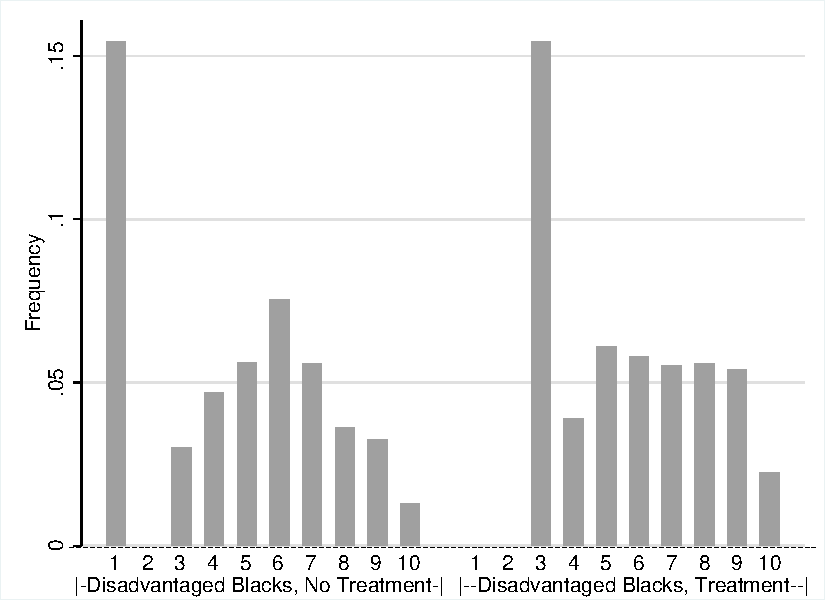
\includegraphics{female1_perry}}} \\
         \subfloat[How the Black Fit into the White Distribution at Age 27, by decile]{
                \scalebox{0.75}{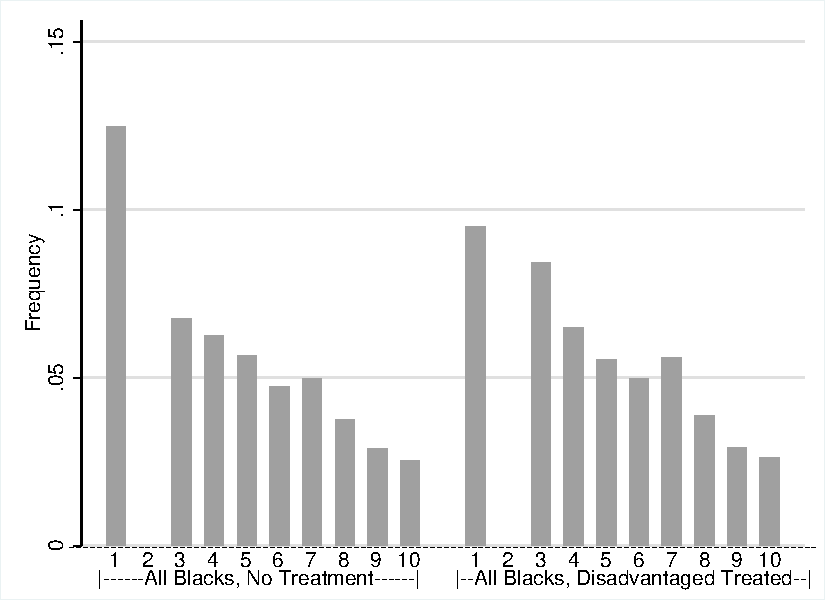
\includegraphics{female2_perry}}} \\
\end{center}
{\scriptsize {\bfseries Notes: } \raggedright The black disadvantaged group is composed of black individuals that satisfy the following criteria: 1) at least one older sibling; 2) IQ score lower than 85; 3) SES index at most 11. All the criteria are measured at age 3. The latter two criteria are approximated as in \citet{heckman2010analyzing}. The black non-disadvantaged are the individuals that violated some of the three criteria above. Black and white are representative of the cohort aged 14-22 in 1979. The left hand side plots consider the cases of the No Action Scenario (Scenario 1): the Perry Program does not influence adult outcomes. The right hand side plots consider cases of the Counter-factual Scenario (Scenario 2): we apply the gender-specific treatment effects of the Perry Program to the disadvantaged black population. We use the treatment effects calculated by \citet{heckman2010analyzing}. 
}
\end{figure}


\begin{figure} \begin{center}\centering
        \caption{Perry Birth Cohort: Total Annual Earnings, Females Age 40}
        \label{female_earn_decile2}\vspace{0.2cm}
         \subfloat[How the Black Disadvantaged Fit into the Black Distribution at Age 40, by decile]{
                \scalebox{0.75}{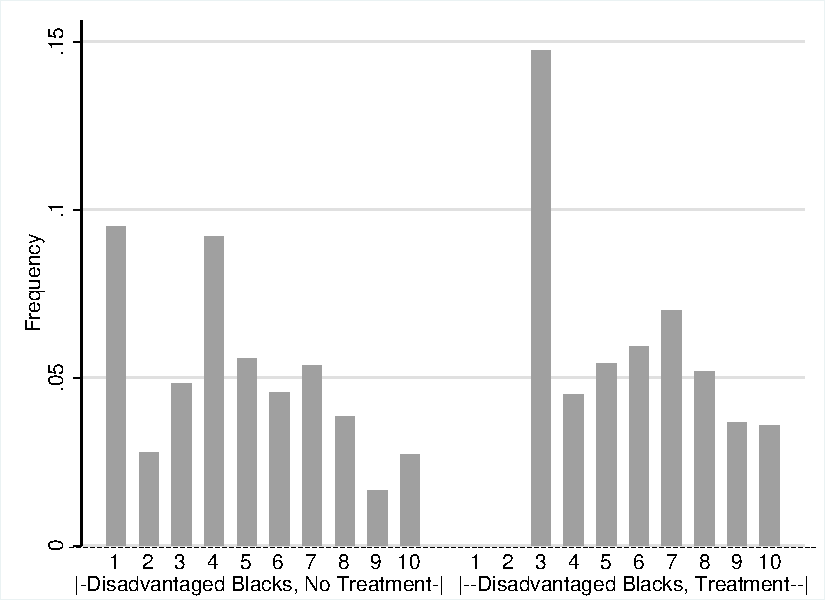
\includegraphics{female3_perry}}} \\
         \subfloat[How the Black Fit into the White Distribution at Age 40, by decile]{
                \scalebox{0.75}{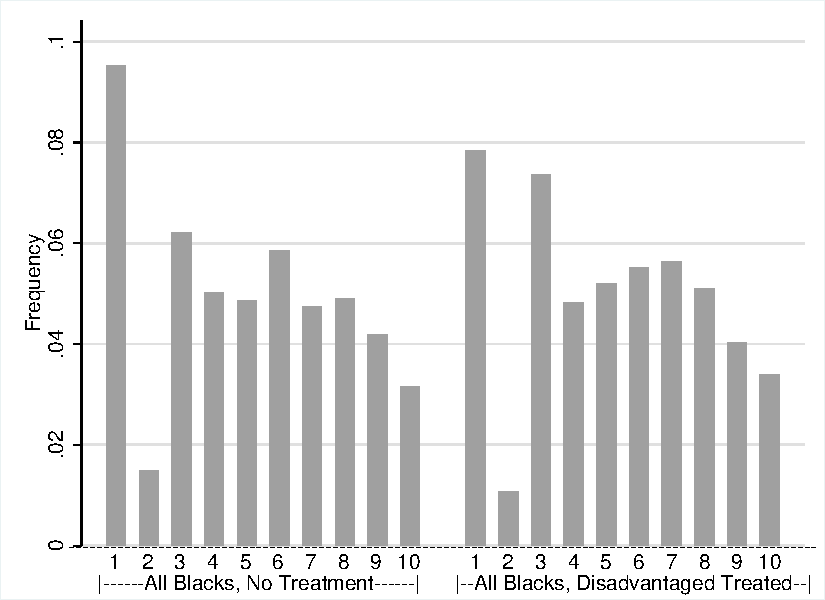
\includegraphics{female4_perry}}} \\     
\end{center}
{\scriptsize {\bfseries Notes: } \raggedright The black disadvantaged group is composed of black individuals that satisfy the following criteria: 1) at least one older sibling; 2) IQ score lower than 85; 3) SES index at most 11. All the criteria are measured at age 3. The latter two criteria are approximated as in \citet{heckman2010analyzing}. The black non-disadvantaged are the individuals that violated some of the three criteria above. Black and white are representative of the cohort aged 14-22 in 1979. The left hand side plots consider the cases of the No Action Scenario (Scenario 1): the Perry Program does not influence adult outcomes. The right hand side plots consider cases of the Counter-factual Scenario (Scenario 2): we apply the gender-specific treatment effects of the Perry Program to the disadvantaged black population. We use the treatment effects calculated by \citet{heckman2010analyzing}. 
}
\end{figure}


\begin{figure} \begin{center}\centering
        \caption{Perry Birth Cohort: Total Annual Earnings, Males Age 27}
        \label{male_earn_decile1}\vspace{0.2cm}
        
         \subfloat[How the Black Disadvantaged Fit into the Black Distribution at Age 27, by decile]{
                \scalebox{0.75}{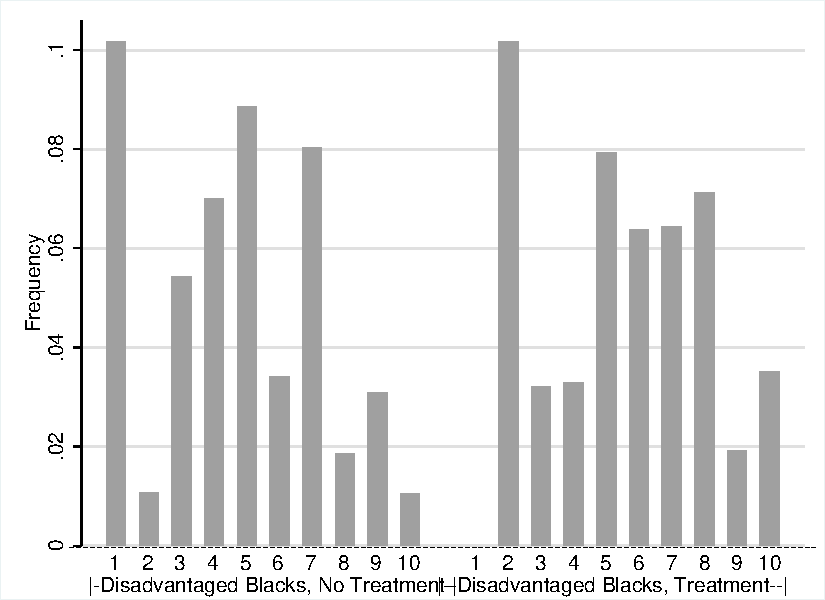
\includegraphics{male1_perry}}} \\
         \subfloat[How the Black Fit into the White Distribution at Age 27, by decile]{
                \scalebox{0.75}{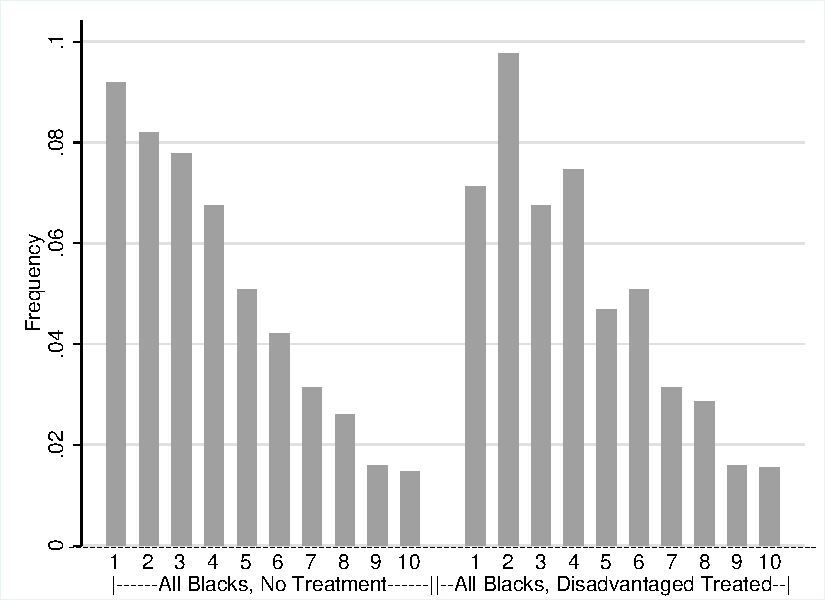
\includegraphics{male2_perry}}} \\
\end{center}
{\scriptsize {\bfseries Notes: } \raggedright The black disadvantaged group is composed of black individuals that satisfy the following criteria: 1) at least one older sibling; 2) IQ score lower than 85; 3) SES index at most 11. All the criteria are measured at age 3. The latter two criteria are approximated as in \citet{heckman2010analyzing}. The black non-disadvantaged are the individuals that violated some of the three criteria above. Black and white are representative of the cohort aged 14-22 in 1979. The left hand side plots consider the cases of the No Action Scenario (Scenario 1): the Perry Program does not influence adult outcomes. The right hand side plots consider cases of the Counter-factual Scenario (Scenario 2): we apply the gender-specific treatment effects of the Perry Program to the disadvantaged black population. We use the treatment effects calculated by \citet{heckman2010analyzing}. 
}
\end{figure}



\begin{figure} \begin{center}\centering
        \caption{Perry Birth Cohort: Total Annual Earnings, Males Age 40}
        \label{male_earn_decile2}\vspace{0.2cm}

         \subfloat[How the Black Disadvantaged Fit into the Black Distribution at Age 40, by decile]{
                \scalebox{0.75}{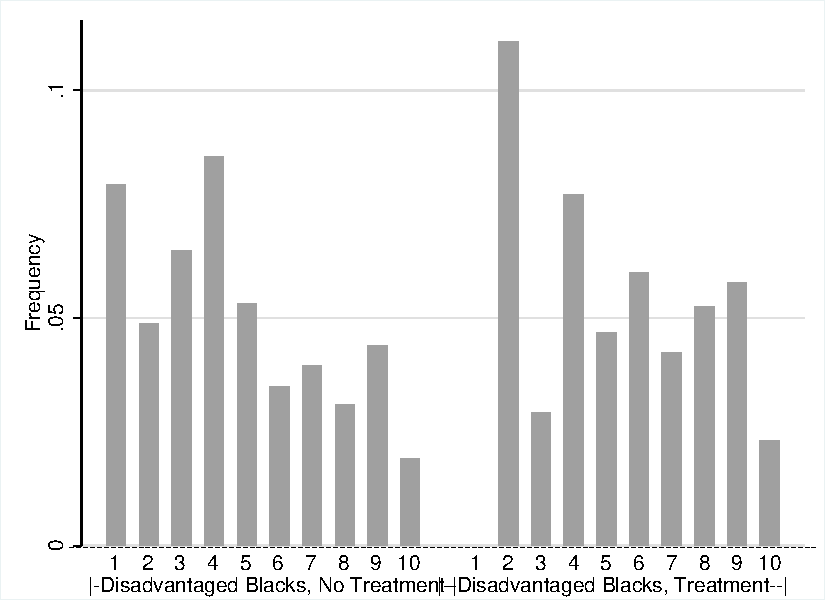
\includegraphics{male3_perry}}} \\
         \subfloat[How the Black Fit into the White Distribution at Age 40, by decile]{
                \scalebox{0.75}{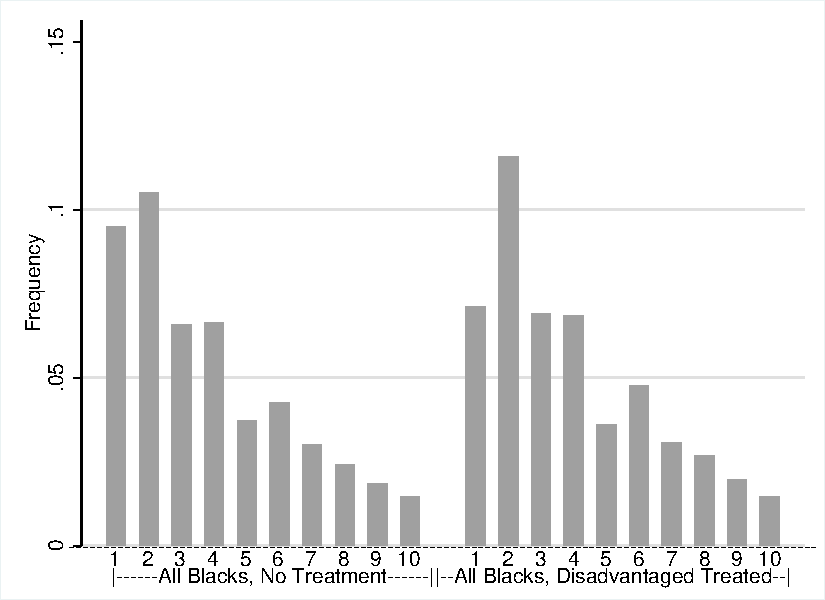
\includegraphics{male4_perry}}} \\ 
\end{center}
{\scriptsize {\bfseries Notes: } \raggedright The black disadvantaged group is composed of black individuals that satisfy the following criteria: 1) at least one older sibling; 2) IQ score lower than 85; 3) SES index at most 11. All the criteria are measured at age 3. The latter two criteria are approximated as in \citet{heckman2010analyzing}. The black non-disadvantaged are the individuals that violated some of the three criteria above. Black and white are representative of the cohort aged 14-22 in 1979. The left hand side plots consider the cases of the No Action Scenario (Scenario 1): the Perry Program does not influence adult outcomes. The right hand side plots consider cases of the Counter-factual Scenario (Scenario 2): we apply the gender-specific treatment effects of the Perry Program to the disadvantaged black population. We use the treatment effects calculated by \citet{heckman2010analyzing}. 
}
\end{figure}


\restoregeometry




%\input{Graphs}

\medskip{}


\medskip{}


